% Options for packages loaded elsewhere
\PassOptionsToPackage{unicode}{hyperref}
\PassOptionsToPackage{hyphens}{url}
%
\documentclass[
]{article}
\usepackage{amsmath,amssymb}
\usepackage{iftex}
\ifPDFTeX
  \usepackage[T1]{fontenc}
  \usepackage[utf8]{inputenc}
  \usepackage{textcomp} % provide euro and other symbols
\else % if luatex or xetex
  \usepackage{unicode-math} % this also loads fontspec
  \defaultfontfeatures{Scale=MatchLowercase}
  \defaultfontfeatures[\rmfamily]{Ligatures=TeX,Scale=1}
\fi
\usepackage{lmodern}
\ifPDFTeX\else
  % xetex/luatex font selection
\fi
% Use upquote if available, for straight quotes in verbatim environments
\IfFileExists{upquote.sty}{\usepackage{upquote}}{}
\IfFileExists{microtype.sty}{% use microtype if available
  \usepackage[]{microtype}
  \UseMicrotypeSet[protrusion]{basicmath} % disable protrusion for tt fonts
}{}
\makeatletter
\@ifundefined{KOMAClassName}{% if non-KOMA class
  \IfFileExists{parskip.sty}{%
    \usepackage{parskip}
  }{% else
    \setlength{\parindent}{0pt}
    \setlength{\parskip}{6pt plus 2pt minus 1pt}}
}{% if KOMA class
  \KOMAoptions{parskip=half}}
\makeatother
\usepackage{xcolor}
\usepackage[margin=1in]{geometry}
\usepackage{graphicx}
\makeatletter
\def\maxwidth{\ifdim\Gin@nat@width>\linewidth\linewidth\else\Gin@nat@width\fi}
\def\maxheight{\ifdim\Gin@nat@height>\textheight\textheight\else\Gin@nat@height\fi}
\makeatother
% Scale images if necessary, so that they will not overflow the page
% margins by default, and it is still possible to overwrite the defaults
% using explicit options in \includegraphics[width, height, ...]{}
\setkeys{Gin}{width=\maxwidth,height=\maxheight,keepaspectratio}
% Set default figure placement to htbp
\makeatletter
\def\fps@figure{htbp}
\makeatother
\setlength{\emergencystretch}{3em} % prevent overfull lines
\providecommand{\tightlist}{%
  \setlength{\itemsep}{0pt}\setlength{\parskip}{0pt}}
\setcounter{secnumdepth}{-\maxdimen} % remove section numbering
\usepackage{fontspec}
\setmainfont{Arial}
\usepackage{booktabs}
\usepackage{longtable}
\usepackage{array}
\usepackage{multirow}
\usepackage{wrapfig}
\usepackage{float}
\usepackage{colortbl}
\usepackage{pdflscape}
\usepackage{tabu}
\usepackage{threeparttable}
\usepackage{threeparttablex}
\usepackage[normalem]{ulem}
\usepackage{makecell}
\usepackage{xcolor}
\ifLuaTeX
  \usepackage{selnolig}  % disable illegal ligatures
\fi
\usepackage{bookmark}
\IfFileExists{xurl.sty}{\usepackage{xurl}}{} % add URL line breaks if available
\urlstyle{same}
\hypersetup{
  pdftitle={dialysistrackR},
  hidelinks,
  pdfcreator={LaTeX via pandoc}}

\title{dialysistrackR}
\author{}
\date{\vspace{-2.5em}2025-06-10}

\begin{document}
\maketitle

\subsection{Introduction}\label{introduction}

This report was generated using a collaborative R Markdown workflow
designed to support transparent, reproducible analysis across sites. The
project is maintained in a shared GitHub repository, with version
tracking, package management, and rendering controlled programmatically
to ensure consistency across contributors and outputs.

The content that follows represents the current state of shared
analysis, with outputs suitable for team review, audit and integration
into clinical workflows.

\subsection{Haemoglobin}\label{haemoglobin}

\begin{table}[!h]
\centering
\caption{\label{tab:plot_function_trend_tables}Most Recent Haemoglobin Results Outside Target Range}
\centering
\begin{tabular}[t]{lcccl}
\toprule
Patient UR & Date & HGB (g/L) & Flag & Trend\\
\midrule
\cellcolor{gray!10}{RB114617} & \cellcolor{gray!10}{08-Jun-2025} & \cellcolor{gray!10}{129.1} & \cellcolor{gray!10}{High} & \cellcolor{gray!10}{NA}\\
RB139157 & 08-Jun-2025 & 120.7 & High & NA\\
\cellcolor{gray!10}{RB143705} & \cellcolor{gray!10}{12-Jun-2025} & \cellcolor{gray!10}{122.2} & \cellcolor{gray!10}{High} & \cellcolor{gray!10}{NA}\\
RB164651 & 11-Jun-2025 & 122.6 & High & NA\\
\cellcolor{gray!10}{RB190135} & \cellcolor{gray!10}{13-Jun-2025} & \cellcolor{gray!10}{136.2} & \cellcolor{gray!10}{High} & \cellcolor{gray!10}{NA}\\
\addlinespace
RB229963 & 10-Jun-2025 & 134.3 & High & ↑ Rising\\
\cellcolor{gray!10}{RB237595} & \cellcolor{gray!10}{09-Jun-2025} & \cellcolor{gray!10}{124.8} & \cellcolor{gray!10}{High} & \cellcolor{gray!10}{↑ Rising}\\
RB239151 & 10-Jun-2025 & 126.9 & High & NA\\
\cellcolor{gray!10}{RB240331} & \cellcolor{gray!10}{10-Jun-2025} & \cellcolor{gray!10}{126.0} & \cellcolor{gray!10}{High} & \cellcolor{gray!10}{NA}\\
RB241413 & 12-Jun-2025 & 122.6 & High & ↑ Rising\\
\addlinespace
\cellcolor{gray!10}{RB266875} & \cellcolor{gray!10}{08-Jun-2025} & \cellcolor{gray!10}{131.2} & \cellcolor{gray!10}{High} & \cellcolor{gray!10}{↑ Rising}\\
RB286230 & 08-Jun-2025 & 120.5 & High & ↑ Rising\\
\cellcolor{gray!10}{RB303077} & \cellcolor{gray!10}{12-Jun-2025} & \cellcolor{gray!10}{130.7} & \cellcolor{gray!10}{High} & \cellcolor{gray!10}{NA}\\
RB308989 & 12-Jun-2025 & 122.0 & High & NA\\
\cellcolor{gray!10}{RB315176} & \cellcolor{gray!10}{12-Jun-2025} & \cellcolor{gray!10}{124.8} & \cellcolor{gray!10}{High} & \cellcolor{gray!10}{↑ Rising}\\
\addlinespace
RB323851 & 09-Jun-2025 & 127.8 & High & NA\\
\cellcolor{gray!10}{RB331216} & \cellcolor{gray!10}{10-Jun-2025} & \cellcolor{gray!10}{133.4} & \cellcolor{gray!10}{High} & \cellcolor{gray!10}{NA}\\
RB344272 & 13-Jun-2025 & 121.1 & High & NA\\
\cellcolor{gray!10}{RB350844} & \cellcolor{gray!10}{07-Jun-2025} & \cellcolor{gray!10}{123.5} & \cellcolor{gray!10}{High} & \cellcolor{gray!10}{NA}\\
RB355256 & 11-Jun-2025 & 126.3 & High & NA\\
\addlinespace
\cellcolor{gray!10}{RB355875} & \cellcolor{gray!10}{11-Jun-2025} & \cellcolor{gray!10}{122.7} & \cellcolor{gray!10}{High} & \cellcolor{gray!10}{NA}\\
RB414403 & 13-Jun-2025 & 131.2 & High & NA\\
\cellcolor{gray!10}{RB439547} & \cellcolor{gray!10}{07-Jun-2025} & \cellcolor{gray!10}{124.6} & \cellcolor{gray!10}{High} & \cellcolor{gray!10}{↑ Rising}\\
RB456797 & 12-Jun-2025 & 129.8 & High & NA\\
\cellcolor{gray!10}{RB473714} & \cellcolor{gray!10}{08-Jun-2025} & \cellcolor{gray!10}{121.5} & \cellcolor{gray!10}{High} & \cellcolor{gray!10}{↓ Falling}\\
\addlinespace
RB477107 & 09-Jun-2025 & 122.9 & High & NA\\
\cellcolor{gray!10}{RB489894} & \cellcolor{gray!10}{11-Jun-2025} & \cellcolor{gray!10}{123.8} & \cellcolor{gray!10}{High} & \cellcolor{gray!10}{↓ Falling}\\
RB497147 & 07-Jun-2025 & 120.3 & High & NA\\
\cellcolor{gray!10}{RB515474} & \cellcolor{gray!10}{11-Jun-2025} & \cellcolor{gray!10}{122.7} & \cellcolor{gray!10}{High} & \cellcolor{gray!10}{NA}\\
RB539953 & 12-Jun-2025 & 124.4 & High & ↑ Rising\\
\addlinespace
\cellcolor{gray!10}{RB540899} & \cellcolor{gray!10}{08-Jun-2025} & \cellcolor{gray!10}{128.0} & \cellcolor{gray!10}{High} & \cellcolor{gray!10}{NA}\\
RB567203 & 09-Jun-2025 & 128.0 & High & ↑ Rising\\
\cellcolor{gray!10}{RB569096} & \cellcolor{gray!10}{08-Jun-2025} & \cellcolor{gray!10}{127.0} & \cellcolor{gray!10}{High} & \cellcolor{gray!10}{NA}\\
RB578001 & 10-Jun-2025 & 124.1 & High & NA\\
\cellcolor{gray!10}{RB580563} & \cellcolor{gray!10}{09-Jun-2025} & \cellcolor{gray!10}{127.0} & \cellcolor{gray!10}{High} & \cellcolor{gray!10}{NA}\\
\addlinespace
RB584475 & 13-Jun-2025 & 120.9 & High & NA\\
\cellcolor{gray!10}{RB601923} & \cellcolor{gray!10}{07-Jun-2025} & \cellcolor{gray!10}{124.0} & \cellcolor{gray!10}{High} & \cellcolor{gray!10}{↑ Rising}\\
RB626085 & 09-Jun-2025 & 120.1 & High & NA\\
\cellcolor{gray!10}{RB638926} & \cellcolor{gray!10}{08-Jun-2025} & \cellcolor{gray!10}{125.3} & \cellcolor{gray!10}{High} & \cellcolor{gray!10}{NA}\\
RB656182 & 09-Jun-2025 & 67.7 & Low & ↓ Falling\\
\addlinespace
\cellcolor{gray!10}{RB683839} & \cellcolor{gray!10}{08-Jun-2025} & \cellcolor{gray!10}{124.3} & \cellcolor{gray!10}{High} & \cellcolor{gray!10}{↑ Rising}\\
RB716617 & 10-Jun-2025 & 120.6 & High & NA\\
\cellcolor{gray!10}{RB725105} & \cellcolor{gray!10}{11-Jun-2025} & \cellcolor{gray!10}{124.4} & \cellcolor{gray!10}{High} & \cellcolor{gray!10}{↑ Rising}\\
RB729679 & 07-Jun-2025 & 136.9 & High & ↑ Rising\\
\cellcolor{gray!10}{RB751053} & \cellcolor{gray!10}{10-Jun-2025} & \cellcolor{gray!10}{129.9} & \cellcolor{gray!10}{High} & \cellcolor{gray!10}{NA}\\
\addlinespace
RB751056 & 11-Jun-2025 & 126.4 & High & NA\\
\cellcolor{gray!10}{RB752587} & \cellcolor{gray!10}{11-Jun-2025} & \cellcolor{gray!10}{121.8} & \cellcolor{gray!10}{High} & \cellcolor{gray!10}{NA}\\
RB770513 & 10-Jun-2025 & 124.3 & High & NA\\
\cellcolor{gray!10}{RB776159} & \cellcolor{gray!10}{10-Jun-2025} & \cellcolor{gray!10}{123.4} & \cellcolor{gray!10}{High} & \cellcolor{gray!10}{NA}\\
RB803272 & 07-Jun-2025 & 123.4 & High & ↑ Rising\\
\addlinespace
\cellcolor{gray!10}{RB820613} & \cellcolor{gray!10}{08-Jun-2025} & \cellcolor{gray!10}{122.5} & \cellcolor{gray!10}{High} & \cellcolor{gray!10}{NA}\\
RB828708 & 13-Jun-2025 & 127.1 & High & NA\\
\cellcolor{gray!10}{RB841991} & \cellcolor{gray!10}{07-Jun-2025} & \cellcolor{gray!10}{120.1} & \cellcolor{gray!10}{High} & \cellcolor{gray!10}{↑ Rising}\\
RB870085 & 13-Jun-2025 & 126.8 & High & ↑ Rising\\
\cellcolor{gray!10}{RB871113} & \cellcolor{gray!10}{09-Jun-2025} & \cellcolor{gray!10}{121.0} & \cellcolor{gray!10}{High} & \cellcolor{gray!10}{↑ Rising}\\
\addlinespace
RB872418 & 08-Jun-2025 & 122.4 & High & ↑ Rising\\
\cellcolor{gray!10}{RB875248} & \cellcolor{gray!10}{10-Jun-2025} & \cellcolor{gray!10}{122.1} & \cellcolor{gray!10}{High} & \cellcolor{gray!10}{↑ Rising}\\
RB887528 & 10-Jun-2025 & 120.2 & High & ↑ Rising\\
\cellcolor{gray!10}{RB899808} & \cellcolor{gray!10}{07-Jun-2025} & \cellcolor{gray!10}{73.7} & \cellcolor{gray!10}{Low} & \cellcolor{gray!10}{↓ Falling}\\
RB904549 & 10-Jun-2025 & 128.2 & High & NA\\
\addlinespace
\cellcolor{gray!10}{RB910149} & \cellcolor{gray!10}{12-Jun-2025} & \cellcolor{gray!10}{120.4} & \cellcolor{gray!10}{High} & \cellcolor{gray!10}{↑ Rising}\\
RB912770 & 09-Jun-2025 & 122.9 & High & ↑ Rising\\
\cellcolor{gray!10}{RB916177} & \cellcolor{gray!10}{09-Jun-2025} & \cellcolor{gray!10}{125.9} & \cellcolor{gray!10}{High} & \cellcolor{gray!10}{NA}\\
RB926217 & 10-Jun-2025 & 122.6 & High & NA\\
\cellcolor{gray!10}{RB935975} & \cellcolor{gray!10}{12-Jun-2025} & \cellcolor{gray!10}{132.0} & \cellcolor{gray!10}{High} & \cellcolor{gray!10}{↑ Rising}\\
\addlinespace
RB949051 & 13-Jun-2025 & 120.7 & High & NA\\
\cellcolor{gray!10}{RB957703} & \cellcolor{gray!10}{11-Jun-2025} & \cellcolor{gray!10}{123.4} & \cellcolor{gray!10}{High} & \cellcolor{gray!10}{NA}\\
RB965052 & 10-Jun-2025 & 127.5 & High & NA\\
\bottomrule
\multicolumn{5}{l}{\textsuperscript{} Trend indicates a change of 10 units as compared to prior result, regardless of date. Only patients with High or Low results are shown.}\\
\end{tabular}
\end{table}

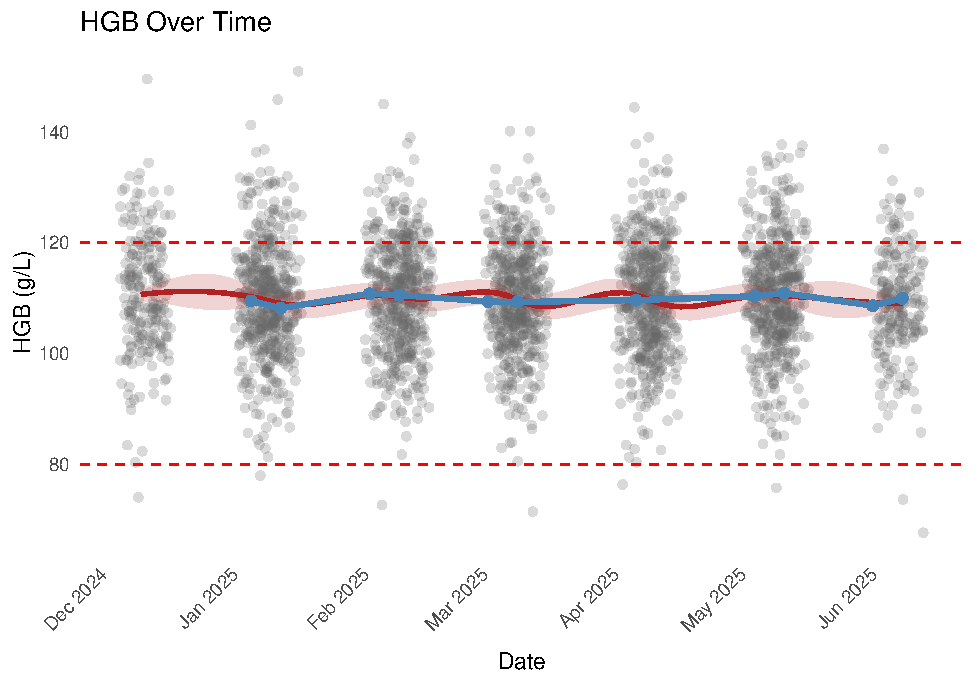
\includegraphics{DialysistrackR_files/figure-latex/plot_function_trend_tables-1.pdf}

\subsection{Interpretation}\label{interpretation}

This plot visualises haemoglobin (HGB) levels across the unit over time.
Unit-level trends can help identify systemic issues affecting multiple
patients --- such as inconsistent access to erythropoiesis-stimulating
agents (ESAs), delays in blood draws, or problems with iron management.

\begin{itemize}
\item
  Raw data (grey dots): Each point represents a single HGB result from
  an individual patient on a specific date, imported directly from
  AUSLAB.
\item
  Red line (LOESS curve): A smoothed estimate of the trend in HGB values
  over time. LOESS (Locally Estimated Scatterplot Smoothing) is a
  nonparametric method that fits multiple small, local regressions to
  the data. It's particularly useful for visualising subtle shifts and
  inflection points without assuming a linear or fixed relationship.
\item
  Pale red area (confidence interval): A 95\% confidence interval around
  the LOESS curve. It gives a visual indication of uncertainty in the
  smoothed trend --- wider areas imply more variability or fewer
  observations at that timepoint.
\item
  Blue line (weekly median): The weekly median HGB, calculated across
  all patients tested in that week. It provides a robust, point-in-time
  summary less sensitive to extreme values than the mean.
\item
  Red dashed lines: The Kidney Health Service's target haemoglobin range
  (80--120 g/L). Values falling persistently outside this band may
  indicate a need for clinical review at the unit or system level.
\end{itemize}

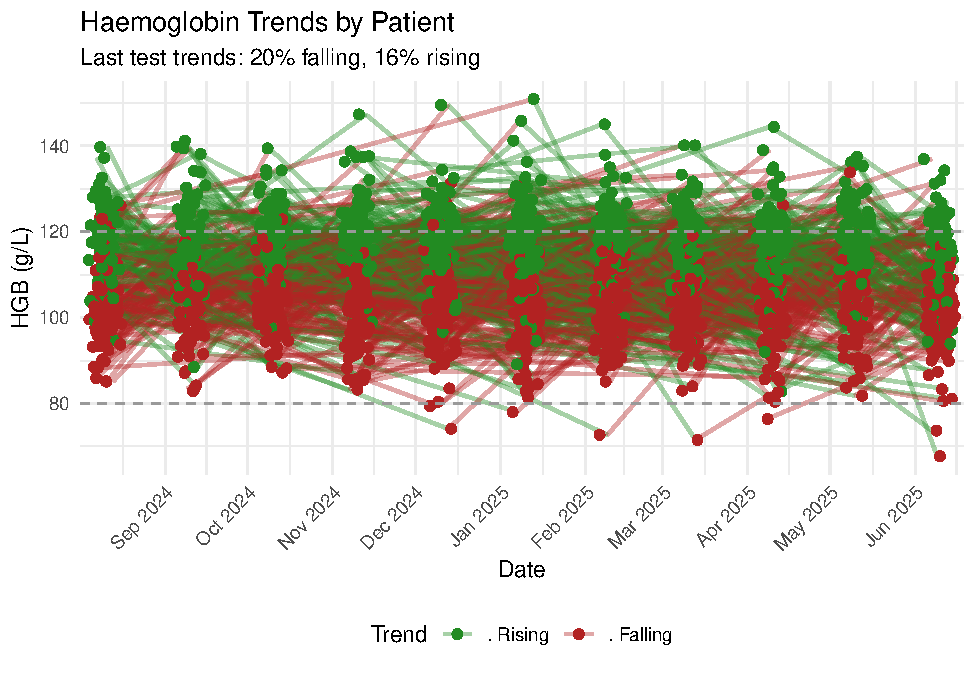
\includegraphics{DialysistrackR_files/figure-latex/Individual_patients-1.pdf}
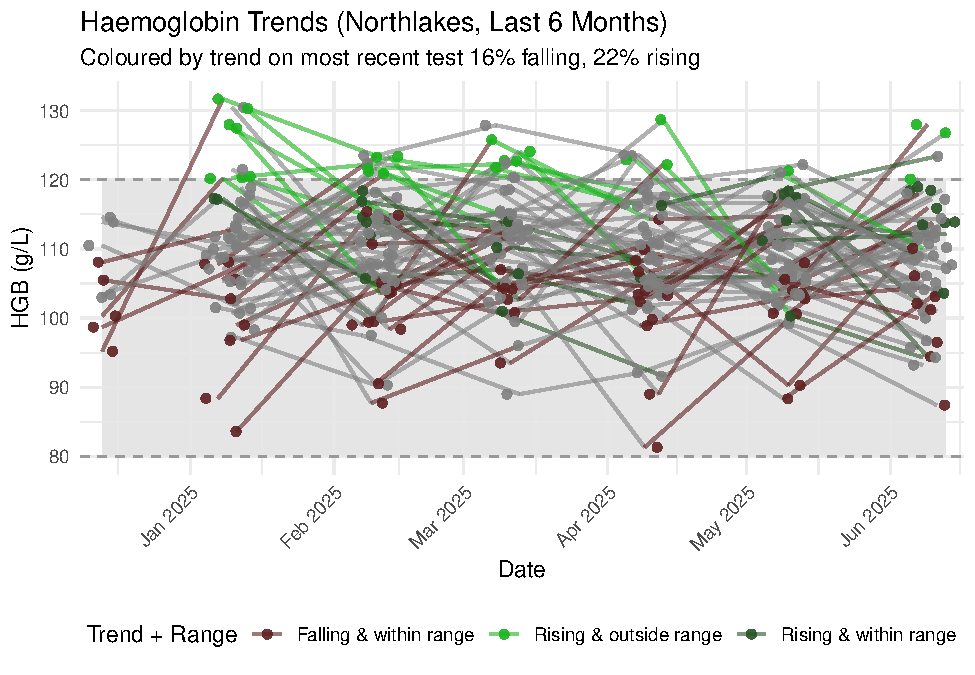
\includegraphics{DialysistrackR_files/figure-latex/Individual_patients-2.pdf}

\begin{table}[!h]
\centering
\caption{\label{tab:Individual_patients}Summary of Most Recent Haemoglobin Results for Subset Patients}
\centering
\begin{tabular}[t]{lcccl}
\toprule
Patient UR & Date & HGB (g/L) & Trend & Trend + Range\\
\midrule
\cellcolor{gray!10}{RB481103} & \cellcolor{gray!10}{13-Jun-2025} & \cellcolor{gray!10}{103.1} & \cellcolor{gray!10}{↓ Falling} & \cellcolor{gray!10}{Falling \& within range}\\
RB822054 & 13-Jun-2025 & 113.9 & ↑ Rising & Rising \& within range\\
\cellcolor{gray!10}{RB870085} & \cellcolor{gray!10}{13-Jun-2025} & \cellcolor{gray!10}{126.8} & \cellcolor{gray!10}{↑ Rising} & \cellcolor{gray!10}{Rising \& outside range}\\
RB961797 & 13-Jun-2025 & 112.2 & NA & Other\\
\cellcolor{gray!10}{RB998806} & \cellcolor{gray!10}{13-Jun-2025} & \cellcolor{gray!10}{107.7} & \cellcolor{gray!10}{NA} & \cellcolor{gray!10}{Other}\\
\addlinespace
RB244397 & 12-Jun-2025 & 103.9 & NA & Other\\
\cellcolor{gray!10}{RB413346} & \cellcolor{gray!10}{12-Jun-2025} & \cellcolor{gray!10}{118.5} & \cellcolor{gray!10}{↑ Rising} & \cellcolor{gray!10}{Rising \& within range}\\
RB501377 & 12-Jun-2025 & 107.2 & NA & Other\\
\cellcolor{gray!10}{RB297793} & \cellcolor{gray!10}{11-Jun-2025} & \cellcolor{gray!10}{87.4} & \cellcolor{gray!10}{↓ Falling} & \cellcolor{gray!10}{Falling \& within range}\\
RB319348 & 11-Jun-2025 & 101.0 & NA & Other\\
\addlinespace
\cellcolor{gray!10}{RB390654} & \cellcolor{gray!10}{11-Jun-2025} & \cellcolor{gray!10}{110.2} & \cellcolor{gray!10}{NA} & \cellcolor{gray!10}{Other}\\
RB603040 & 11-Jun-2025 & 114.4 & NA & Other\\
\cellcolor{gray!10}{RB640405} & \cellcolor{gray!10}{11-Jun-2025} & \cellcolor{gray!10}{112.7} & \cellcolor{gray!10}{NA} & \cellcolor{gray!10}{Other}\\
RB934681 & 11-Jun-2025 & 103.6 & ↑ Rising & Rising \& within range\\
\cellcolor{gray!10}{RB957703} & \cellcolor{gray!10}{11-Jun-2025} & \cellcolor{gray!10}{123.4} & \cellcolor{gray!10}{NA} & \cellcolor{gray!10}{Other}\\
\addlinespace
RB168582 & 10-Jun-2025 & 113.8 & ↑ Rising & Rising \& within range\\
\cellcolor{gray!10}{RB327568} & \cellcolor{gray!10}{10-Jun-2025} & \cellcolor{gray!10}{96.5} & \cellcolor{gray!10}{↓ Falling} & \cellcolor{gray!10}{Falling \& within range}\\
RB698384 & 10-Jun-2025 & 96.7 & NA & Other\\
\cellcolor{gray!10}{RB791855} & \cellcolor{gray!10}{10-Jun-2025} & \cellcolor{gray!10}{117.2} & \cellcolor{gray!10}{NA} & \cellcolor{gray!10}{Other}\\
RB854246 & 10-Jun-2025 & 111.9 & NA & Other\\
\addlinespace
\cellcolor{gray!10}{RB957782} & \cellcolor{gray!10}{10-Jun-2025} & \cellcolor{gray!10}{101.2} & \cellcolor{gray!10}{↓ Falling} & \cellcolor{gray!10}{Falling \& within range}\\
RB227191 & 09-Jun-2025 & 115.9 & ↑ Rising & Rising \& within range\\
\cellcolor{gray!10}{RB363765} & \cellcolor{gray!10}{09-Jun-2025} & \cellcolor{gray!10}{108.4} & \cellcolor{gray!10}{NA} & \cellcolor{gray!10}{Other}\\
RB567203 & 09-Jun-2025 & 128.0 & ↑ Rising & Rising \& outside range\\
\cellcolor{gray!10}{RB631378} & \cellcolor{gray!10}{09-Jun-2025} & \cellcolor{gray!10}{104.1} & \cellcolor{gray!10}{NA} & \cellcolor{gray!10}{Other}\\
\addlinespace
RB689835 & 09-Jun-2025 & 94.4 & ↓ Falling & Falling \& within range\\
\cellcolor{gray!10}{RB693898} & \cellcolor{gray!10}{09-Jun-2025} & \cellcolor{gray!10}{111.7} & \cellcolor{gray!10}{NA} & \cellcolor{gray!10}{Other}\\
RB765436 & 09-Jun-2025 & 111.4 & NA & Other\\
\cellcolor{gray!10}{RB930049} & \cellcolor{gray!10}{09-Jun-2025} & \cellcolor{gray!10}{109.0} & \cellcolor{gray!10}{NA} & \cellcolor{gray!10}{Other}\\
RB130759 & 08-Jun-2025 & 112.1 & NA & Other\\
\addlinespace
\cellcolor{gray!10}{RB380638} & \cellcolor{gray!10}{08-Jun-2025} & \cellcolor{gray!10}{118.4} & \cellcolor{gray!10}{↑ Rising} & \cellcolor{gray!10}{Rising \& within range}\\
RB644601 & 08-Jun-2025 & 106.1 & NA & Other\\
\cellcolor{gray!10}{RB645747} & \cellcolor{gray!10}{08-Jun-2025} & \cellcolor{gray!10}{93.2} & \cellcolor{gray!10}{NA} & \cellcolor{gray!10}{Other}\\
RB650813 & 08-Jun-2025 & 102.1 & ↓ Falling & Falling \& within range\\
\cellcolor{gray!10}{RB677480} & \cellcolor{gray!10}{08-Jun-2025} & \cellcolor{gray!10}{105.1} & \cellcolor{gray!10}{NA} & \cellcolor{gray!10}{Other}\\
\addlinespace
RB750127 & 08-Jun-2025 & 94.3 & NA & Other\\
\cellcolor{gray!10}{RB833880} & \cellcolor{gray!10}{08-Jun-2025} & \cellcolor{gray!10}{113.5} & \cellcolor{gray!10}{↑ Rising} & \cellcolor{gray!10}{Rising \& within range}\\
RB936631 & 08-Jun-2025 & 110.1 & ↓ Falling & Falling \& within range\\
\cellcolor{gray!10}{RB986113} & \cellcolor{gray!10}{08-Jun-2025} & \cellcolor{gray!10}{106.1} & \cellcolor{gray!10}{↓ Falling} & \cellcolor{gray!10}{Falling \& within range}\\
RB100887 & 07-Jun-2025 & 108.9 & NA & Other\\
\addlinespace
\cellcolor{gray!10}{RB104146} & \cellcolor{gray!10}{07-Jun-2025} & \cellcolor{gray!10}{110.8} & \cellcolor{gray!10}{NA} & \cellcolor{gray!10}{Other}\\
RB125094 & 07-Jun-2025 & 95.7 & NA & Other\\
\cellcolor{gray!10}{RB295892} & \cellcolor{gray!10}{07-Jun-2025} & \cellcolor{gray!10}{113.3} & \cellcolor{gray!10}{NA} & \cellcolor{gray!10}{Other}\\
RB346794 & 07-Jun-2025 & 104.3 & NA & Other\\
\cellcolor{gray!10}{RB455582} & \cellcolor{gray!10}{07-Jun-2025} & \cellcolor{gray!10}{108.8} & \cellcolor{gray!10}{NA} & \cellcolor{gray!10}{Other}\\
\addlinespace
RB505468 & 07-Jun-2025 & 104.4 & NA & Other\\
\cellcolor{gray!10}{RB758417} & \cellcolor{gray!10}{07-Jun-2025} & \cellcolor{gray!10}{119.0} & \cellcolor{gray!10}{↑ Rising} & \cellcolor{gray!10}{Rising \& within range}\\
RB800576 & 07-Jun-2025 & 118.0 & NA & Other\\
\cellcolor{gray!10}{RB841991} & \cellcolor{gray!10}{07-Jun-2025} & \cellcolor{gray!10}{120.1} & \cellcolor{gray!10}{↑ Rising} & \cellcolor{gray!10}{Rising \& outside range}\\
RB870419 & 07-Jun-2025 & 100.0 & NA & Other\\
\bottomrule
\end{tabular}
\end{table}

\subsubsection{Patient level Hb
interpretation}\label{patient-level-hb-interpretation}

This plot displays haemoglobin (HGB) levels over time for individual
patients, each represented by a connected line. Colours reflect the
direction of change based on their most recent result: - Red indicates a
downward trend (↓ Falling) - Green indicates an upward trend (↑ Rising)

The dashed grey lines represent target HGB thresholds (80--120 g/L). The
background band highlights the target range. Most patients remain within
or near target, but as of the most recent test: 16\% show a falling
trend, 22\% show a rising trend, and 0\% are stable. , This plot
displays haemoglobin (HGB) levels over time for individual patients,
each represented by a connected line. Colours reflect the direction of
change based on their most recent result: - Red indicates a downward
trend (↓ Falling) - Green indicates an upward trend (↑ Rising)

The dashed grey lines represent target HGB thresholds (80--120 g/L). The
background band highlights the target range. Most patients remain within
or near target, but as of the most recent test: NA show a falling trend,
NA show a rising trend, and NA are stable.

This figure shows longitudinal haemoglobin (HGB) results for 50 patients
at the Northlakes unit over the past six months. Each line represents an
individual patient trajectory, coloured by both the direction of trend
and whether the most recent result was within the target range.

\begin{itemize}
\tightlist
\item
  Green: Rising HGB
\item
  Red: Falling HGB
\item
  Grey: Stable HGB
\item
  Brighter colours indicate a most recent value outside the 80--120 g/L
  target range; muted colours indicate values within range.
\end{itemize}

As of the most recent measurement: - 16\% of patients were trending
downward - 22\% were trending upward - 0\% were stable

The shaded region indicates the HGB target range (80--120 g/L). This
visual supports identification of patients who may benefit from anaemia
review or intervention.

\subsection{Haemoglobin Results
tabulated}\label{haemoglobin-results-tabulated}

\begin{verbatim}
## Above Target    |  66 patients |  13.2%
## Below Target    |   2 patients |   0.4%
## Within Target   | 432 patients |  86.4%
\end{verbatim}

\begin{verbatim}
## Patients who dropped from ≥80 to <80 g/L within 30 days:  2
\end{verbatim}

\begin{verbatim}
## Patients with ≥10 g/L HGB drop within 30 days:  45
\end{verbatim}

\begin{longtable}[t]{llrrrrl}
\caption{\label{tab:hgb_analysis}Most Recent Flagged Haemoglobin Event per Patientm within 30 days}\\
\toprule
Ur Number & CollectedDate & HGB & prev\_HGB & delta\_HGB & delta\_days & Event\\
\midrule
RB100562 & 2025-06-07 & 100.1 & 124.4 & -24.3 & 28 & Drop ≥10 g/L in ≤30 days\\
RB113934 & 2025-06-07 & 97.3 & 115.3 & -18.0 & 26 & Drop ≥10 g/L in ≤30 days\\
RB194355 & 2025-06-11 & 107.3 & 118.9 & -11.6 & 29 & Drop ≥10 g/L in ≤30 days\\
RB243348 & 2025-06-08 & 102.7 & 117.1 & -14.4 & 27 & Drop ≥10 g/L in ≤30 days\\
RB274978 & 2025-06-08 & 102.6 & 115.7 & -13.1 & 26 & Drop ≥10 g/L in ≤30 days\\
\addlinespace
RB280510 & 2025-06-07 & 101.4 & 128.9 & -27.5 & 29 & Drop ≥10 g/L in ≤30 days\\
RB286230 & 2025-05-13 & 103.0 & 113.0 & -10.0 & 30 & Drop ≥10 g/L in ≤30 days\\
RB319594 & 2025-06-07 & 92.5 & 115.8 & -23.3 & 28 & Drop ≥10 g/L in ≤30 days\\
RB340449 & 2025-06-10 & 107.9 & 123.6 & -15.7 & 28 & Drop ≥10 g/L in ≤30 days\\
RB366988 & 2025-06-09 & 116.7 & 127.5 & -10.8 & 29 & Drop ≥10 g/L in ≤30 days\\
\addlinespace
RB382387 & 2025-06-08 & 90.7 & 114.0 & -23.3 & 27 & Drop ≥10 g/L in ≤30 days\\
RB383059 & 2025-05-11 & 110.5 & 125.7 & -15.2 & 30 & Drop ≥10 g/L in ≤30 days\\
RB407159 & 2025-06-08 & 109.0 & 122.0 & -13.0 & 28 & Drop ≥10 g/L in ≤30 days\\
RB413543 & 2025-05-12 & 88.6 & 100.1 & -11.5 & 29 & Drop ≥10 g/L in ≤30 days\\
RB422330 & 2025-06-10 & 105.8 & 121.5 & -15.7 & 28 & Drop ≥10 g/L in ≤30 days\\
\addlinespace
RB434193 & 2025-06-07 & 105.5 & 122.3 & -16.8 & 25 & Drop ≥10 g/L in ≤30 days\\
RB482545 & 2025-06-07 & 101.5 & 115.9 & -14.4 & 26 & Drop ≥10 g/L in ≤30 days\\
RB489894 & 2025-06-11 & 123.8 & 137.5 & -13.7 & 30 & Drop ≥10 g/L in ≤30 days\\
RB494805 & 2025-06-09 & 113.0 & 135.4 & -22.4 & 30 & Drop ≥10 g/L in ≤30 days\\
RB495643 & 2025-06-10 & 92.1 & 111.2 & -19.1 & 28 & Drop ≥10 g/L in ≤30 days\\
\addlinespace
RB497573 & 2025-06-08 & 99.4 & 117.2 & -17.8 & 30 & Drop ≥10 g/L in ≤30 days\\
RB507757 & 2025-06-09 & 101.9 & 116.8 & -14.9 & 27 & Drop ≥10 g/L in ≤30 days\\
RB539531 & 2025-06-08 & 96.4 & 113.6 & -17.2 & 26 & Drop ≥10 g/L in ≤30 days\\
RB548924 & 2025-05-11 & 102.5 & 114.0 & -11.5 & 29 & Drop ≥10 g/L in ≤30 days\\
RB557080 & 2025-06-09 & 106.0 & 121.5 & -15.5 & 29 & Drop ≥10 g/L in ≤30 days\\
\addlinespace
RB570329 & 2025-06-08 & 97.5 & 118.0 & -20.5 & 27 & Drop ≥10 g/L in ≤30 days\\
RB650813 & 2025-06-08 & 102.1 & 117.5 & -15.4 & 29 & Drop ≥10 g/L in ≤30 days\\
RB656182 & 2025-06-09 & 67.7 & 117.5 & -49.8 & 29 & Drop from ≥80 to <80 g/L\\
RB659205 & 2025-06-11 & 105.3 & 122.0 & -16.7 & 30 & Drop ≥10 g/L in ≤30 days\\
RB692286 & 2025-06-09 & 101.8 & 113.0 & -11.2 & 28 & Drop ≥10 g/L in ≤30 days\\
\addlinespace
RB693593 & 2025-06-07 & 104.0 & 115.8 & -11.8 & 28 & Drop ≥10 g/L in ≤30 days\\
RB702000 & 2025-06-10 & 110.9 & 129.1 & -18.2 & 28 & Drop ≥10 g/L in ≤30 days\\
RB721953 & 2025-06-11 & 94.5 & 113.7 & -19.2 & 29 & Drop ≥10 g/L in ≤30 days\\
RB733965 & 2025-06-10 & 97.1 & 109.8 & -12.7 & 28 & Drop ≥10 g/L in ≤30 days\\
RB743987 & 2025-06-08 & 95.4 & 106.8 & -11.4 & 27 & Drop ≥10 g/L in ≤30 days\\
\addlinespace
RB747230 & 2025-06-12 & 92.3 & 108.5 & -16.2 & 30 & Drop ≥10 g/L in ≤30 days\\
RB873405 & 2025-06-07 & 106.9 & 135.3 & -28.4 & 27 & Drop ≥10 g/L in ≤30 days\\
RB875307 & 2025-05-11 & 106.3 & 119.6 & -13.3 & 30 & Drop ≥10 g/L in ≤30 days\\
RB888483 & 2025-06-12 & 94.0 & 112.0 & -18.0 & 30 & Drop ≥10 g/L in ≤30 days\\
RB889034 & 2025-06-11 & 107.6 & 118.5 & -10.9 & 30 & Drop ≥10 g/L in ≤30 days\\
\addlinespace
RB899808 & 2025-06-07 & 73.7 & 95.4 & -21.7 & 26 & Drop from ≥80 to <80 g/L\\
RB914660 & 2025-06-12 & 109.1 & 122.4 & -13.3 & 30 & Drop ≥10 g/L in ≤30 days\\
RB925979 & 2025-06-11 & 107.6 & 122.1 & -14.5 & 29 & Drop ≥10 g/L in ≤30 days\\
RB930533 & 2025-06-09 & 116.6 & 129.5 & -12.9 & 30 & Drop ≥10 g/L in ≤30 days\\
RB957782 & 2025-06-10 & 101.2 & 116.4 & -15.2 & 29 & Drop ≥10 g/L in ≤30 days\\
\addlinespace
RB985173 & 2025-06-07 & 103.4 & 122.3 & -18.9 & 26 & Drop ≥10 g/L in ≤30 days\\
RB986113 & 2025-06-08 & 106.1 & 121.0 & -14.9 & 29 & Drop ≥10 g/L in ≤30 days\\
\bottomrule
\end{longtable}

\section{Target Summary}\label{target-summary}

\begin{verbatim}
## HGB
## no. of pts >= 80: 1
## no. of pts <= 115: 1
## TRFSAT
## no. of pts >= 20: 1
## no. of pts <= 50: 1
## K
## no. of pts >= 3: 1
## no. of pts <= 5.5: 1
## PTHR
## no. of pts >= 18: 1
## no. of pts <= 90: 1
## PHOS
## no. of pts >= 1.5: 1
## no. of pts <= 4: 1
## CAL
## no. of pts >= 2: 1
## no. of pts <= 2.6: 1
## ALB
## no. of pts >= 20: 1
## no. of pts <= 40: 1
\end{verbatim}

\section{Transferrin Saturation}\label{transferrin-saturation}

\section{Serum Potassium}\label{serum-potassium}

\section{Serum Parathyroid Hormone}\label{serum-parathyroid-hormone}

\section{Serum Phosphate}\label{serum-phosphate}

\section{Serum Calcium}\label{serum-calcium}

\section{Serum Albumin}\label{serum-albumin}

\section{Hepatitis B Serum
Antibodies}\label{hepatitis-b-serum-antibodies}

\end{document}
